\documentclass{article}
\usepackage{enumerate}
\usepackage{amsmath}
\usepackage{amssymb}
\usepackage{graphicx}
\usepackage{subfigure}
\usepackage{geometry}
\usepackage{caption}
\usepackage{indentfirst}

\usepackage{tikz}
\usetikzlibrary{circuits.ee.IEC}
\usetikzlibrary{arrows.meta}
\usetikzlibrary{calc}

\usepackage{minted}

\geometry{left=3.0cm,right=3.0cm,top=3.0cm,bottom=4.0cm}
\renewcommand{\thesection}{Problem \arabic{section}.}
%\allowdisplaybreaks[4]
\newcommand{\Omegacm}{{\rm\,\Omega\cdot cm}}
\newcommand{\unit}[1]{{\rm\,#1}}

\title{VE311 Homework 9}
\author{Liu Yihao 515370910207}
\date{}

\begin{document}
\maketitle

\section{}
\begin{figure}[!htbp]
\centering
\subfigure[$R_D=1k\Omega$]{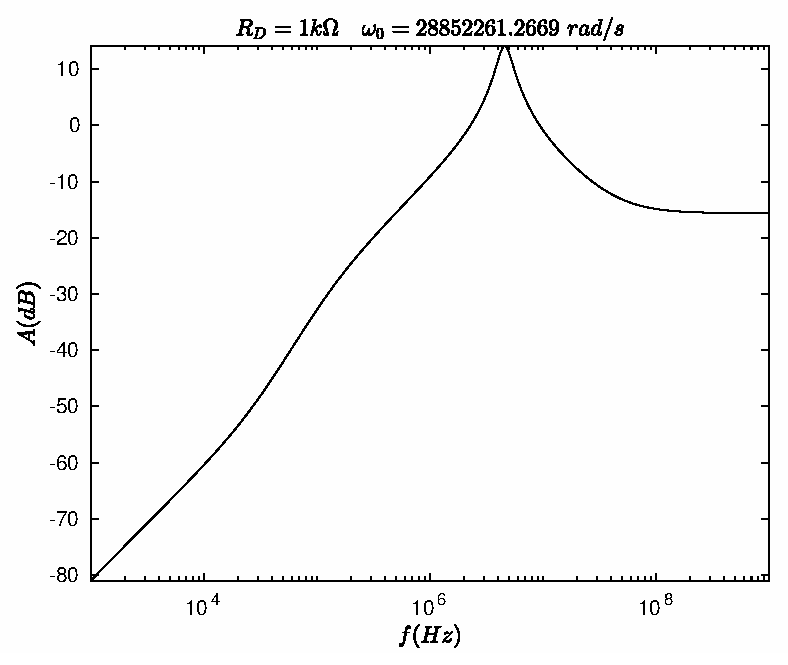
\includegraphics[width=0.32\linewidth]{p1_0.eps}}
\subfigure[$R_D=10k\Omega$]{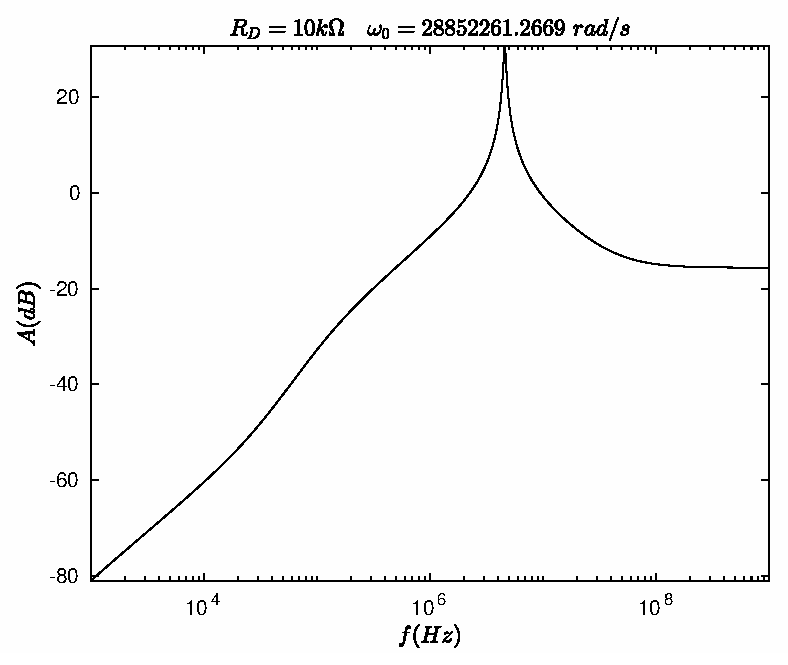
\includegraphics[width=0.32\linewidth]{p1_1.eps}}
\subfigure[$R_D=100k\Omega$]{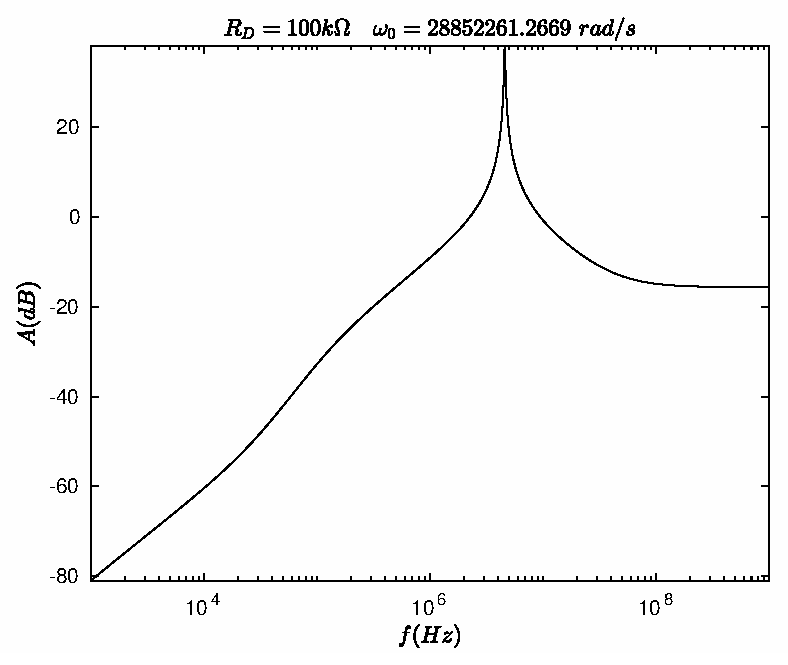
\includegraphics[width=0.32\linewidth]{p1_2.eps}}
\subfigure[$R_D=500k\Omega$]{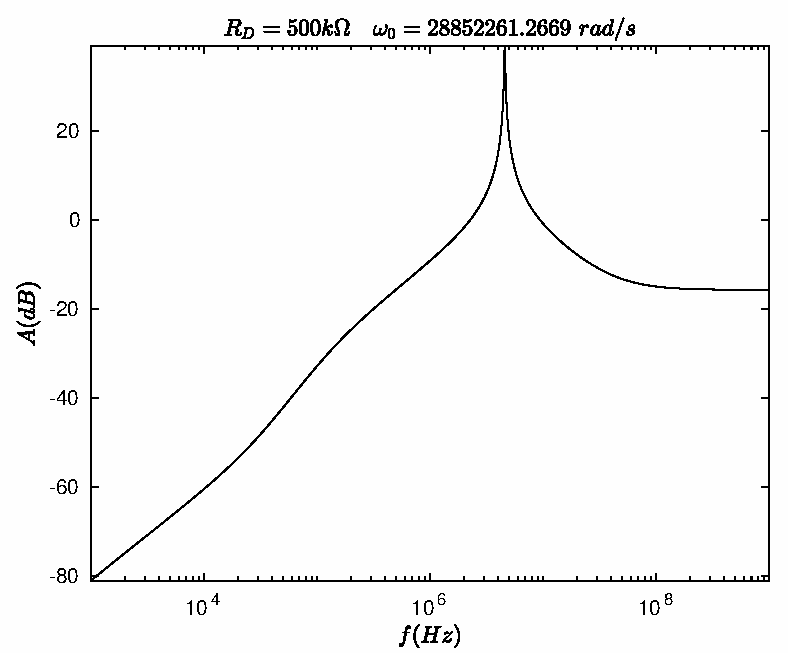
\includegraphics[width=0.32\linewidth]{p1_3.eps}}
\subfigure[$R_D=1M\Omega$]{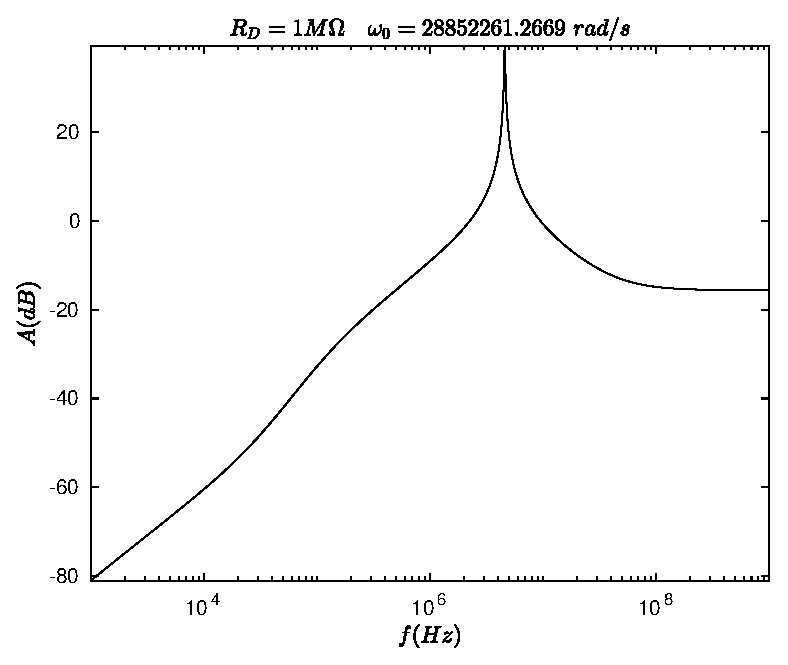
\includegraphics[width=0.32\linewidth]{p1_4.eps}}
\caption{Output response different values of $R_D$.}
\label{fig1-1}
\end{figure}

In Figure \ref{fig1-1}, We can find that $\omega_0=28.852\unit{Mrad/s}$ in different values of $R_D$. There is also a figure of all resistances (Figure \ref{fig1-2}), in which we can find that the larger $R_D$ is, the larger the output response.

\begin{figure}[!htbp]
\centering
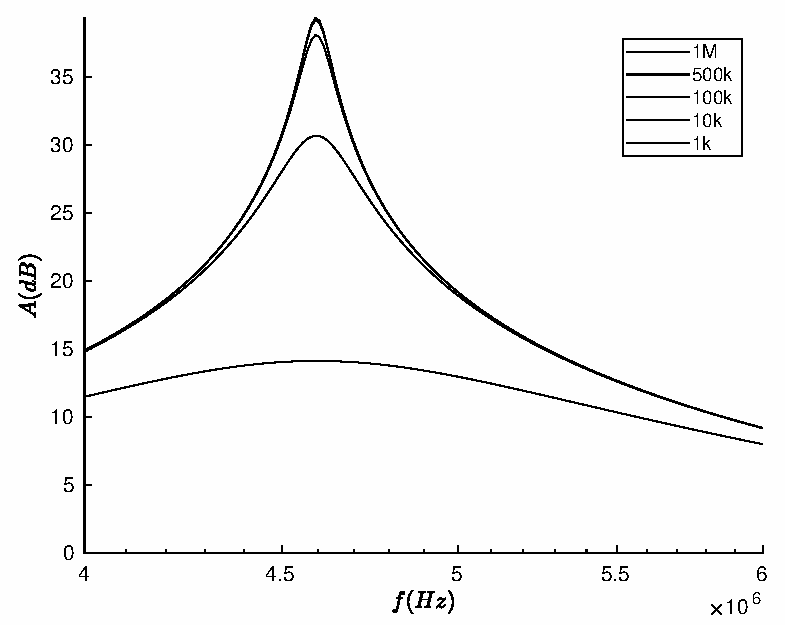
\includegraphics[width=0.6\linewidth]{p1.eps}
\caption{Output response different values of $R_D$ in one graph.}
\label{fig1-2}
\end{figure}

The spice code is

[p1.cir.head]
\inputminted[linenos,xleftmargin=1.5em]{v}{p1.cir.head}

[p1.cir.tail]
\inputminted[linenos,xleftmargin=1.5em]{v}{p1.cir.tail}

The shell code is

\inputminted[linenos,xleftmargin=1.5em]{shell}{p1.sh}

The MATLAB code is

\inputminted[linenos,xleftmargin=1.5em,breaklines]{matlab}{p1.m}


\section{}
\begin{align*}
L(s)&=\left(1+\frac{R_4}{R_3}\right)\cdot\frac{Z_p}{Z_p+Z_s}\\
&=\left(1+\frac{R_4}{R_3}\right)\cdot\frac{1/C_1s\parallel R_1}{1/C_1s\parallel R_1+1/C_2s+R_2}\\
&=\left(1+\frac{R_4}{R_3}\right)\cdot\frac{R_1C_2s}{R_1R_2C_1C_2s^2+(R_1C_1+R_1C_2+R_2C_2)s+1}\\
L(j\omega)&=\left(1+\frac{R_4}{R_3}\right)\cdot\frac{R_1C_2j\omega}{-R_1R_2C_1C_2\omega^2+(R_1C_1+R_1C_2+R_2C_2)j\omega+1}
\end{align*}
$$\left\{\begin{aligned}
&\omega=2000\pi\unit{rad/s}\\
&R_1=R_2,R_4=10\unit{k\Omega}\\
&C_1=0.1\unit{\mu F},C_2=0.22\unit{\mu F}\\
&-R_1R_2C_1C_2\omega^2+1=0\\
&\left(1+\frac{R_4}{R_3}\right)\cdot\frac{R_1C_2}{R_1C_1+R_1C_2+R_2C_2}=1
\end{aligned}\right.\Longrightarrow\left\{\begin{aligned}
R_1&=1.073\unit{k\Omega}\\
R_2&=1.073\unit{k\Omega}\\
R_3&=6.875\unit{k\Omega}
\end{aligned}\right.$$

\section{}



\end{document}

